\documentclass[fleqn]{article}
\usepackage{lipsum} 
\usepackage{manyeqns}
\usepackage{amsmath}
\setlength{\mathindent}{0.5cm}
\usepackage{soul}
\usepackage{color}
\usepackage{eurosym}
\usepackage{natbib}
\usepackage[sc]{mathpazo} % Use the Palatino font
\usepackage[T1]{fontenc} % Use 8-bit encoding that has 256 glyphs
\linespread{1.05} % Line spacing - Palatino needs more space between lines
\usepackage{microtype} % Slightly tweak font spacing for aesthetics
\usepackage{rotating}
\usepackage[hmarginratio=1:1,top=32mm,columnsep=20pt]{geometry} % Document margins
\usepackage{multicol} % Used for the two-column layout of the document
\usepackage{multirow}
\usepackage{hyperref} % For hyperlinks in the PDF

\usepackage[hang, small,labelfont=bf,up,textfont=it,up]{caption} % Custom captions under/above floats in tables or figures
\usepackage{booktabs} % Horizontal rules in tables
\usepackage{float} % Required for tables and figures in the multi-column environment - they need to be placed in specific locations with the [H] (e.g. \begin{table}[H])

\usepackage{lettrine} % The lettrine is the first enlarged letter at the beginning of the text
\usepackage{paralist} % Used for the compactitem environment which makes bullet points with less space between them

\usepackage{graphicx}
\usepackage[FIGBOTCAP]{subfigure}
\usepackage{multirow, booktabs}

\usepackage{abstract} 
\renewcommand{\abstractnamefont}{\normalfont\bfseries} % Set the "Abstract" text to bold
\renewcommand{\abstracttextfont}{\normalfont\small\itshape}
%\citestyle{nSIE}

\usepackage{titlesec} % Allows customization of titles
\renewcommand\thesection{\Roman{section}}
\titleformat{\section}[block]{\large\scshape\centering}{\thesection.}{1em}{} % Change the look of the section titles


\usepackage{fancyhdr} % Headers and footers
\pagestyle{fancy} % All pages have headers and footers
\fancyhead{} % Blank out the default header
\fancyfoot{} % Blank out the default footer
\fancyhead[C]{Paper for review} % Custom header text
\fancyfoot[RO,LE]{\thepage} % Custom footer text

\begin{document}

\title{\vspace{-5mm}\fontsize{14pt}{10pt}\selectfont\textbf{Management of Deteriorating Avalanche Protection Structures using a Time Dependence Replacement Model}} % Article title
\author{
\large
\textrm{Nam Lethanh$^{a}$}\thanks{Corresponding author: lethanh@ibi.baug.ethz.ch or namkyodai@gmail.com} \hspace{2mm} and \textrm{Bryan T. Adey$^{b}$} % Your name
}
\date{}
\maketitle
\textrm{$^{a}$ Research Associate, Dr. Institute of Construction and Infrastructure Management, Swiss Federal Institute of Technology (ETHZ), Zurich, Switzerland} \\ % Your institution
\textrm{$^{b}$ Professor, Institute of Construction and Infrastructure Management, Swiss Federal Institute of Technology (ETHZ), Zurich, Switzerland} \\ % Your institution

\thispagestyle{fancy}

\begin{abstract}
Management of avalanche protection infrastructure requires consideration of the probability of occurrence of failure and its consequences. If a failure occurs consequences are often large as avalanches, rockfalls, and debris flows will hit other infrastructure objects and case drastic reductions in the levels of service provided, until all infrastructure is restored. The risk related to such hazards depends on the probability of occurrence and what happens between the moment an adequate level of service is not provided and it is restored.

To minimize the risk related to avalanche protection infrastructure, managers can execute preventive interventions. For example, an avalanche protection structure can be replaced on regular intervals to reduce the probability of it failing due to heavy snow loads next winter. Such interventions are required as the avalanche protection, as all infrastructure, deteriorate over time, and, therefore, its ability to restrain snow loads, rock falls, and debris flows decreases over time. Obviously the shorter the renewal period the lower the mean number of failures, and therefore, corrective interventions. As the preventive interventions are not free, there is an optimal renewal period, i.e. a renewal period that results in the lowest overall costs. 

In this paper, a block replacement model is used to determine the optimal intervention strategy for avalanche protection structure. The model is tested with an empirical study on an avalanche protection structure where a concrete-steel hybrid bridge may be hit by an avalanche if it occurs. 
\bigskip

{\bf Keywords:} Infrastructure management, Optimal intervention strategy, Hazard risk, Block replacement model, Avalanche protection structures.\bigskip
\end{abstract}

%%%%%%%%%%%%%%%%%%%%%%%%%%%%%%%%%%%%

\section{Introduction} \label{sec1}
\subsection{Management of avalanche protection structure-an overview}
Avalanche is a commom type of natural hazards in mountainous regions. The occurrence of avalanches creates fear and uncertainties, particularly in regions that own critical infrastructure structures and have high density of population. Among the most effects of avalanche, a concrete effect is the restriction of movement, closed road links and bridges, and sometimes isolation of entire communities \citep{Norem1994}. 

Examples of avalanches are vastly docummented, In Norway, each winter, there are about 200-300 avalanches that block the road links while they are openned for free traffic flows \citep{Norem1994}. In Swiss Alps regions, many roads are closed during the winter period and many mountain trains have had to stop operation when avalanches occur. In some serious cases, avalanches can cause loss of life and damage properties, forest, and wildlife \citep{Rudolf-Miklau2011}. 

To prevent avalanches from occurring or to minimize the risk that is might create, avalanche protection structures (APS) are installed on or off the starting zones of avalanches \citep{Sauermoser2011}. As being constructed in areas exposing to extreme weather condition, sometimes unpredicted, the reliability of the APS is in question and it is important for manager to monitor and measure it frequently so as they can pro-actively execute preventive interventions to minimize the risk of structural failures.

Maintenance works on the APS include two types of interventions. One is corrective intervention (CI) that is executed after knowing the APS has failed or its reliability has reached to a critical level. The other is preventive intervention (PI) which is executed at a future time, when managers believe that by executing the PI, the reliability of the APS will be again high and the APS will provides an adequate level of service \citep{Rudolf-Miklau2008,Rudolf-Miklau2011}. The execution of a PI will reduce the risk of having structural failure of the APS and thus minimize the risk of having danger to the society.

To date, research literature on the method to determine the optimal PI for the APS is very limited. Most of the works has focused mainly on the aspects concerning the design, construction, and the CI for the APS \citep{Agerer2007,Rudolf-Miklau2008,Rudolf-Miklau2011,Margreth2007,ONR2010}. Pioneer works on determining the optimal PI can be with the works of \cite{Rudolf-Miklau2008} and \cite{Rudolf-Miklau2011}. In the cited works, the authors discussed the importance of having a life cycle engineering approach in order to come up with an optimal intervention strategy. However, they work was only limited to discussion and illustration of managerial framework but did not specify or recommend a good set of modeling approach to make a rigorous solution to the question. 

In order to determine an optimal PI for the APS, it is important to take into account of consequences of hazards (e.g. avalanches, rockfalls, and debris flows) a community has to be suffered during and after the events beside the consideration of impacts of the CI on the APS itself. In addition, it is also necessary to appropriately estimate the reliability of the APS and the critical infrastructure structures that are affected by the event of avalanches. %This approach is similar to what has been done for management of other engineering systems such as management of bridge, road network, and tunnel. However, there should be some degrees of differences with respect to which is a suitable set of modeling approach and how to quantify or measure the impacts in the case of avalanche occurrence.

\subsection{Research on management of structures affecting by natural hazards}
Assessing and managing hazard risks due to natural disasters have emerged and attracted a great attention in the field of infrastructure asset management in recent years. This is due to the fact that natural disasters could cause a great amount of negative impacts on our modern societies, especially on the utilization of infrastructure network, which is vital to provide an adequate level of services to the people and socio-economic activities. Evidences of the negative consequences of natural disasters on infrastructures are numerous, e.g. the great Tohoku earthquake in Japan in 2011 \citep{Nishiyama2012}, the hurricanes in the USA \citep{Cruz2008,Kates2006,Litman2006}, the rockfalls and snow avalanches on the Alps \citep{Perret2006, Stoffel2005}. 

Research efforts toward building managerial frameworks, models, and methods to assess and mitigate natural hazard risks have been significantly advanced. Most of natural hazard risks are considered as extreme events and their occurrences over time can be assessed through the use of statistical modeling approach. For example, earthquake occurrence can be modeled by Poisson process \citep{Korup2009}. Risks incurred along the infrastructure network can also be predicted using Bayesian network modeling and GIS-tools \citep{Graf2009, Baruffini2010, Noetzli2003}.

With regard to impacts of risks on civil structures, the majority of research has been focusing on the use of fragility curves \citep{Karim2001, Choi2004, Mayet2002}, which represent the failure probability given a certain intensity measure of hazard, e.g. the collapse probability of a concrete building under the occurrence of an earthquake with a magnitude of 7; or the probability of going to failure from any physical condition state of a concrete bridge under the rock falls in mountainous region \citep{Lethanh2013}. Other probabilistic models to account for the failure probability of infrastructure objects can be with exponential distributed family, which includes Poisson distribution, exponential distribution, Weibull distribution, and Gamma distribution \citep{Madanat1995, Lethanh2012b, Cox1959, Davis1952, gertsbakh97}.

The consequences on civil structures once hazards occur cannot be observed beforehand, and thus, the processes that leads to the consequences are considered as latent deterioration process (LDP). This process is different from the process that causes the civil structures to deteriorate gradually, e.g. the corrosion process of steel elements of a bridge or the wear out of asphalt surface on a road section. Such gradual deterioration process can be considered as observable due to manifest deterioration process (MDP) \citep{Lethanh2013}.

To the authors knowledge, despite the fact that there have been a considerable number of researches on risk modeling for predicting hazard events and for assessing the reliability of civil structures, existing models in infrastructure asset management field have not integrated the LDP in the determination of the optimal intervention strategies (OISs). Examples of existing models used in practice are the bridge management systems like the PONTIS and BRIDGIT used in the USA, Canada, and Italy, etc \citep{pontis, Thompson1998, Fruguglietti2012}, the KUBA-MS used in Switzerland \citep{Hajdin2003, ASTRA2010}. In the cited frameworks, only the MDP is considered, i.e. the physical and performance of bridge elements are classified into several discrete condition states, which are not at all representing the failure states under occurrences of hazard events \citep{Mayet2002, Lethanh2013}.

With a broad picture of risk modeling and limitation of state-of-the-art infrastructure management systems (IMSs) as a backdrop, it is necessary now to proceed to fill in carefully the foundations of the IMSs. Some theoretical works on integrating the LDP into existing IMSs have actually been published \citep{Mayet2002, Lethanh2013}. In the cited works, the authors discussed the extension of currently used Markov models in existing IMSs to take the LDP into consideration. The proposed models in the cited papers can be applied in a macroscopic management level. However, the models are still faced with some limitations such as the lack of discount factor in their formulation, or the use of steady state probability.

\subsection{Rationale}
In this paper, it is foreseen that infrastructure managers need to make decisions on the time to execute a periodic intervention (or preventive intervention) for the APS located in hazard region at a regular basic (hereafter referred as time dependence replacement intervention strategy). The APS is undergone latent deterioration process (e.g. reliability decrease due to the sudden impacts of avalanches or rockfalls). If the structure cannot withstand the impacts of avalanches, avalanches could continue to slide down and directly affecting other critical infrastructure structures (CIS) such as road links and bridges. The immediate impact of avalanche is the shutdown of service of the CIS. Traffic route could be closed for days. Furthermore, the CIS can fail to provide adequate level of services and they need an immediate corrective intervention. This scenario is true to many practical situations and in some context it is referred as cascading events. This means, an event occurs that leads to another events and therefore solution to the original event must be located in the context of system instead of individual.

The failure of the CIS due to avalanches depends on its reliability or its condition state at the time of avalanche occurrence. If the reliability is low, there is higher probability that it will fail compared to that when its reliability is high and vise versa. The CIS such as roads, tunnels, and bridges, is undergone two types of deterioration processes. One is the manifest deterioration, which can be measurred gradually and the other is latent process, which cannot be measurred gradually but having to estimate through an engineering approach using the concept of fragility curve.

The question on how to determine the optimal time to execute a PI has been solved in numerous studies on preventive replacement models in operations research (\cite{gertsbakh97, Gertsbakh2000, Kaio1984, Chen1992, Berg1978}). However, non of them focused on extending their models to encompass the cascading events or implicitly perform a numerical solution in the context of infrastructure asset management. 

By taking an advantage of the novel idea from the past research, in this paper, a replacement model developed by \cite{Kaio1984} was selected for further investigation. In the cited work, the authors proposed a replacement model for infinite management of an one-unit system. Their model was initially designed for facility and machinery management alike. Precisely, it is assumed that an object is replaced at failure and exchanged at a time specified a period, respectively. The setup of the model fits naturally the mentioned problem in infrastructure management. It includes the discount factor that is not discussed in many works which only focus on preventive intervention of short life cycle objects (\cite{gertsbakh97}). It proposes a solution for infinite time management of objects, which is relatively suitable for infrastructure structures with a long service life and its cycle of intervention and operation can be assumed with steady state. 

Based on the solid background of the work of \cite{Kaio1984}, this paper is oriented to extend the model and fit it into the context of management of avalanche protection structures and cascading effects possibly triggerred by avalanches. The contributions of the paper are as follows:

\begin{itemize}
	\item Extending the model of \cite{Kaio1984} for the APS with assumption that the reliability of the APS follows a Weibull function,
	\item Developing a connection between the optimization model and the concept of fragility curve, and the Markov deterioration model to estimate the reliability of the CIS,
	\item Presenting the usefulness of the model by means of a numerical example, which was unfortunately missing in the original work of \cite{Kaio1984}.
	\item Performing a rigorous sensitivity analysis in order to highlight some important findings and conclusions that are useful for infrastructure managers when they have to deal with practical situations.
\end{itemize}

The paper is organized as follows: the following section briefly lays out the formulation of the time dependent replacement model. Section \ref{sec3} outlines an example using the model in consideration of the latent deteriotion process, where the reliability of the APS is assessed by Weibull distribution function and the reliability of the CIS is estimated by both manifest and latent processes. In this section, a brief explanation on how to use the fragility curve is also presented. The sensitivity analysis is discussed in Section \ref{sa}. The last section concludes the paper with some highlights on its usefulness and applicability.
%
\section{The block replacement model} \label{sec2}
It is assumed that a preventive intervention (PI) is executed after a pre-defined time $n\cdot T$ ($n=0,1,2,\cdots,N$). Once the PI is executed, the functionality and serviceability of the structure could be the same or different from that of the structure before the intervention. In between the time $\Delta t$ ($[0\le \Delta t \le T]$), hazards could occur and cause the structure in damage states (hereafter denoted as $i$ ($i=1,\cdots,I$)), in which the structure is no longer providing an adequate level of services (l.o.s). In both cases, when the PI or CI is executed, there are impacts incurred by stakeholders $s$ (e.g. the owner, the users, the public).

Following notations are used to describe the formulation of the model.


\begin{tabular}{lp{12.5cm}}
$\theta(\Delta t|t)$ & Conditional failure rate $i$ $(i=1,\cdots,I)$ when the structure has been in service in an interval $t$ after the PI \\ 
$\Psi(\cdot|t)$ & Any conditional function $\Psi$ given that a PI is executed by a unit of age $t$, where $t$ is a random variable \\ 
$F(t)$ & Cumulative distribution function (cdf) of age $t$ of a unit for a PI at execution time\\ 
$w_{p}^s(t)$ & Impacts incurred by stakeholder $s$ due to the execution of PI\\ 
$w_{c}^s(t)$ & Impacts incurred by stakeholder $s$ due to the execution of CI \\ 
$w_o^s(\Delta t|t)$ & Conditional impacts incurred by stakeholder $s$ when the structure is remains in normal operation (\emph{i.e.} providing an adequate level of service) during time interval $\Delta t$ after a PI has been carried out and the structure has not entered failure state\\ 
$\rho$ & discount factor\\
$p_l^k (t)$ & probability of failure at time $t$ of the affecting objects $k$ (e.g. bridge, road)\\
$C_c^{s,k}$ & Impacts incurred by stakeholder $s$ due to the execution of an CI on objects $k$ \\
$T$ & interval between the PIs\\ 
$T^{\star}$ & Optimal interval time between PIs, which is the variable of the model\\
$\Omega_{p}(T,t)$ & minimum expected total discounted impact for an infinite time span when the structure has been in service during an interval $t$ after the execution of the PI and the structure has not entered failure state\\
$\Omega_{c}(T,t)$ & minimum expected total discounted impact for an infinite time span when a CI has been executed, of the structure that has been in service during a time interval $t$ after the execution of the PI and the structure has entered failure state\\
\end{tabular}
In the model, it is assumed that at each damage level $i$, there exists a corresponding well defined CI. Within an increment of time $\Delta t$, after the structure has been under the PI after time $t$, the total expected impacts due to the execution of CIs are:
\begin{eqnarray}
&& v_c (\Delta t|t) =\sum_{s=1}^{S} \left [ w_{c}^s  (\Delta t) + \sum_{k=1}^K p_l^k \cdot C_c^{s,k} \right ] \cdot \theta (\Delta t|t) .\label{totalCIs}
\end{eqnarray}
The total impacts due to the execution of PIs and the total impacts incurred by stakeholders during the service time of the structure are defined in Eq. (\ref{totalPIs}) and Eq. (\ref{totalO}), respectively.
\begin{eqnarray}
&& v_p (t) =\sum_{s=1}^{S}w_{p}^s (t)  .\label{totalPIs}
\end{eqnarray}
\begin{eqnarray}
&& v_o (t) =\sum_{s=1}^{S}w_{o}^s (t)  .\label{totalO}
\end{eqnarray}
According to the principle of optimality, which is described in \citet[p. 15]{Bellman1962}, the minimum expected total discounted impact $\Omega_{c}(T,t)$ for infinite time is formulated in following equation.
\begin{eqnarray}
&& \Omega_{c}(T,t) = \int_0^{\infty} \left[ {v_c(\Delta t|t)} + \Omega_{p}(T,\Delta t|t)  \right] dF(t).\label{omegaCI1}
\end{eqnarray}
The minimum expected total discounted impact $ \Omega_{p}(T,\Delta t|t) $, which appears inside Eq. (\ref{totalCIs}), is obtained as follows
\begin{eqnarray}
&& \Omega_{p}(T,\Delta t) = min \Gamma (\Delta t) .\label{omegaPI1}
\end{eqnarray}
where $\Gamma (\Delta t)$ is defined as
\begin{eqnarray}
&& \Gamma (\Delta t) = \int_0^{\infty} \left[ v_o \int_0^{dt} exp(-\rho \tau)d\tau  + \left\{ {1-\theta(\Delta t|t)dt} \right\}\cdot \Omega_p(T,\Delta t+dt|t) exp(-\rho dt) \right. \nonumber \\
&&  \hspace{20mm} +  \theta(\Delta t|t)dt \cdot \Omega_c(T,\Delta t+dt|t)exp(-\rho dt) \left.\vphantom{\int_t} \right] dF(t).\label{gamma1}
\end{eqnarray}
According to \citet{Kaio1984}, Eq. (\ref{gamma1}) is rewritten in following form
\begin{eqnarray}
&& \Gamma (\Delta t) = \Omega_{p}(T,\Delta t) + \left[ -\rho \Omega_{p}(T,\Delta t) +d\Omega_{p}(T,\Delta t)/dt \right]dt \nonumber \\
&& \hspace{30mm} + \int_0^{\infty} \left[ v_o + v_c(\Delta t|t) \right]dF(t)dt.\label{gamma2}
\end{eqnarray}
Thus, from $\Omega_p(T,\Delta t)=\Gamma(\Delta t)$ (Eq. (\ref{omegaPI1})), the following equation can be derived:
\begin{eqnarray}
&& \Omega_p(T,\Delta t) = exp(\rho\Delta t) \left[\Omega_p(T,0)-\int_0^{\infty}\int_0^t exp(-\rho\tau) \left\{ v_o+v_c(\tau|t)\right\} \right]d\tau dF(t)
.\label{omegaPI2}
\end{eqnarray}
where,
\begin{eqnarray}
&& \Omega_p(T,0) = \left\{1-exp(-\rho T)\right\}^{-1} \int_0^{\infty} \left[ \vphantom{\int_t} exp(-\rho T) \left\{ v_p(T,t) \right\} \right. \nonumber \\
&& \hspace{45mm}+ \int_0^T exp(-\rho \Delta t) \left\{ v_o (\Delta t|t) + v_c(\Delta t|t) \right\} dt \left.\vphantom{\int_t} \right] dF(t).\label{omegaPI3}
\end{eqnarray}
when $T$ tends to infinity $T \to \infty $, Eq. (\ref{omegaPI3}) becomes
\begin{eqnarray}
&& \Omega_p(\infty,0) = \int_0^{\infty}\int_0^{\infty}exp(-\rho t) \left[v_o + v_c(\Delta t|t) \right] dt dF(t).\label{omegaPI4}
\end{eqnarray}
Eqs. (\ref{omegaPI3}) and (\ref{omegaPI4}) are the explicit forms of the expected total discounted impact in infinite time horizon. This is the classical optimization problem. By differentiating the expected total discounted impact $\Omega_p(T,0)$ and $\Omega_p(\infty,0)$ and setting it equal to zero, the optimal time $T^{\star}$ can be obtained. 
The optimal time $T^{\star}$ for PI is the solution of the following system of equations:
\begin{eqnarray}
&& \left\{ {\begin{array}{*{20}{c}}
 {{T^{\star}} = \arg \mathop {\min }\limits_{{T^{\star}} \in [0,T]} {\Theta _p}(T,0)}\\
 {{T^{\star}} = \arg \mathop {\min }\limits_{{T^{\star}} \in [0,\infty ]} {\Theta _p}(\infty ,0)}
\end{array}} \right. 
\end{eqnarray}
in which the differentiates of $\Theta_p(T,0)$ and $\Theta_p(\infty,0)$ are respectively:
\begin{eqnarray}
&& \Theta_p(T,0)  = \frac{\delta (\Omega_p(T,0))}{\delta T} \nonumber \\
&& \hspace{14mm} = \left[1-exp(-\rho T) \right] \int_0^{\infty} \left[ \vphantom{\int_t} -\rho v_p(T,t) \right. \nonumber \\
&& \hspace{20mm} +d(v_p(T,t))/dT + v_o(T,t) + v_p(T,t) \left.\vphantom{\int_t}\right]dF(t) \nonumber \\
&& \hspace{20mm} -\rho \int_0^{\infty} \left[ \vphantom{\int_t} exp(-\rho T)\left\{v_p(T,t) \right\}\right. \nonumber \\
&& \hspace{20mm}  +\int_0^T exp(-\rho \Delta t) \left\{v_o(\Delta t|t) + v_c(\Delta t|t) \right\} dt \left.\vphantom{\int_t}\right] dF(t).\label{omegaPI5}
\end{eqnarray}
and
\begin{eqnarray}
&& \Theta_p(\infty,0)  = \frac{\delta (\Omega_p(\infty,0))}{\delta T} \nonumber \\
&& \hspace{14mm} = \int_0^{\infty} \left[-\rho \left\{v_p(\infty|t)+ \int_0^{\infty}exp(-\rho t) \left\{v_o(\Delta t|t)+ v_p(\Delta t|t)  \right\}\right\} \right. \nonumber \\
&& \hspace{20mm} + \mathop {\lim }\limits_{T \to \infty } d(v_p(T,t))/dT + v_o(\infty|t) + v_p(\infty|t) \left.\vphantom{\int_t}\right] dF(t) \label{omegaPI6}
\end{eqnarray}

\section{Illustrative example} \label{sec3}
% % %
\subsection{General}
The case study is formulated for two types of structures. One is a system of snow barriers installed on a side rocky mountain above the road link. The other is a two-lanes steel concrete hybrid bridge located underneath the rocky mountain. Due to the topology of the area, there is a high risk that snow-packs can be formed in the starting zones and avalanches can occur. If the system of the snow barriers fails to prevent an avalanche or a rockfall from occurring, the bridge will be in direct danger, i.e. there is a probability that the bridge can be no longer provide an adequate level of service for an amount of time.

In order to minimize such as risk of avalanche occurrence, the system of snow barriers needs to be replaced (preventive intervention) after a certain period of time in service. The replacement of the snow barriers system will ensure that its reliability is always at highest degree possible and results in lowest impacts to the bridge and hence to all stakeholders.

% \begin{figure}[H]
%   \begin{center}
%   \subfigure[snow barriers system]
%   	{
%     \includegraphics[width=0.45\linewidth]{snowbarriers}
%     }
%   \subfigure[hybrid steel bridge]
%     {
%       \includegraphics[width=0.45\linewidth]{steelbridge}
%       }
%     \caption{Illustration of objects in case study}
%     \label{objectscasestudy}
%   \end{center}
% \end{figure}

Without loss of generality, it is assumed that the PI incurs a total of 1 monetary unit (mu). The impacts of the CI on the snow-barrier system is considered as X mus and on the bridge is Y mus, respectively. Values of X and Y will be selected with precise numbers for illustrative purpose. They are also used for sensitivity analysis. It is important at this outset of the calculation to mention that it is not necessary to demonstrate the usefulness of the model with a real case study since, from mathematical point of view, the determination of optimal IOS is dependent mainly on the ratio between the PI and CI once the reliability of the APS and the CIS are determined. 

However, it is necessary to briefly discuss on how to compute the value of PI and CI for the barrier system and for the bridge in a real application work. Values of PI and CI are, in principle, estimated from various sources. For example, they can be an approximate values that infrastructure managers were suffered from execution of the past intervention work. Both CI and PI are considered as total sum of impacts incurred to all stakeholders during the course of executing them. For example, the value of an CI for the bridge under failure situation should includes all impacts incurred to local residents, users who might loose time for traveling in case of an avalanche hits the bridge and the bridge has to be closed. 

% A brief overview of the snow barriers system and the bridge is given in Table \ref{exampleoverview}.

% \begin{table}[htbp]
% \caption{Overview of the snow barriers system and the bridge}
% \begin{center}
% \begin{tabular}{|l|c|c|}
% \hline
% \textbf{Description} & \textbf{Snow barriers system} & \textbf{Bridge} \\ \hline
% Number of objects & 20 & 1 \\ \hline
% Width of an object & x & x \\ \hline
% Length of an object & x & x \\ \hline
% Materials & Steel & Hybrid steel \\ \hline
% Capacity & 29 KN/m3 & 100 train/day \\ \hline
% \end{tabular}
% \end{center}
% \label{exampleoverview}
% \end{table}

\subsection{Reliability assumption}
\subsubsection{Reliability of the snow barriers system}
To simplify the calculation while still keeping the breath of the content, it is assumed that the reliability of the snow barriers system follows a Weibull distribution function. This function is appropriately used as it considers the time-dependent latent deterioration process. Following equations briefly show the hazard function, probability density function, and the reliability function for the snow barriers system.
\begin{manyeqns}
&& \lambda(\tau) = \alpha \cdot m \cdot \tau^{m-1} \label{eq14} \\
&& f(\tau) = \alpha \cdot m \cdot \tau^{m-1} \cdot e^{-(\alpha \tau)^m} \label{eq15}\\
&& F(\tau) = 1-e^{-(\alpha \tau)^m} \label{eq16}
\end{manyeqns}

Values of $\alpha$ and $m$ are assumed to be $0.0252$ and $1.2665$, respectively. This assumption is used, again, for illustrative purpose only. Later, in sensitivity analysis section, they are varied to see the changes in the optimal time to execute PI. Under this assumption, once can construct the reliability curves as shown in Figure \ref{reliability-snowbarriers}.

\begin{figure}[H]
  \begin{center}
    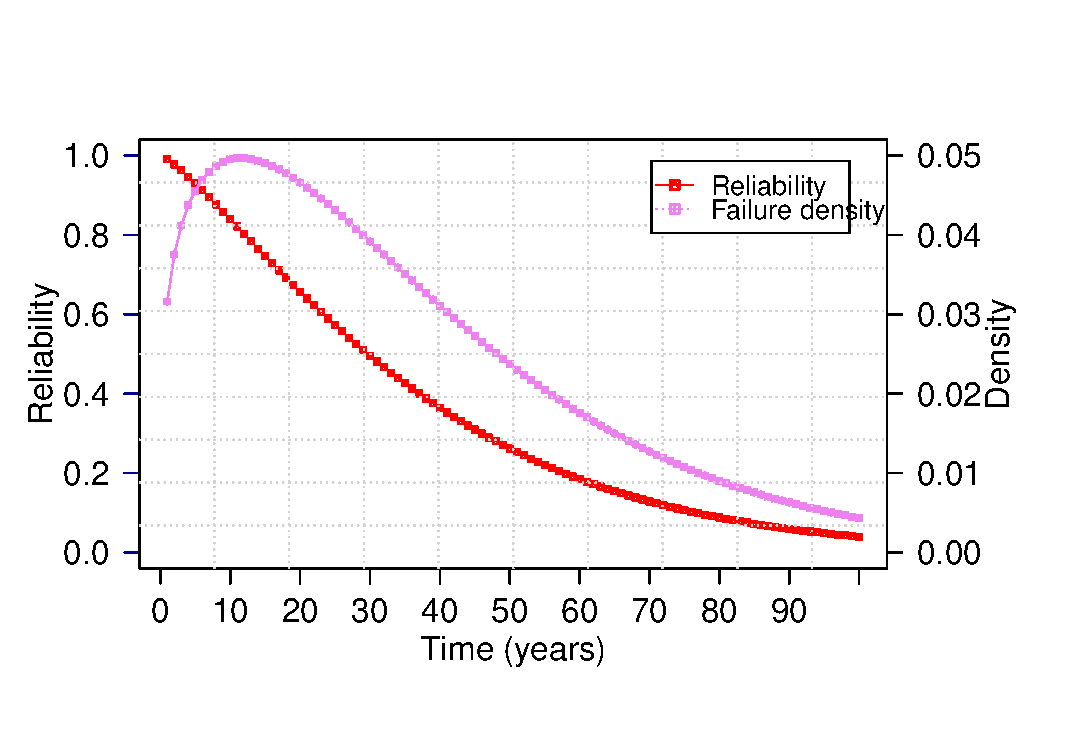
\includegraphics[width=0.8\linewidth]{reliability-snowbarriers}
    \caption{ Reliability curves of snow-barrier systems}
    \label{reliability-snowbarriers}
  \end{center}
\end{figure}

The reliability curves shows a gradual decrease in the reliability of the snow-barrier system over time. More or less after 25 years, the reliability of the system will reduce to about 50\%. 

\subsubsection{Reliability of the bridge}
On the other hands, the reliability of the bridge is estimated using the concept of fragility curve, which is dependent on actual state of the bridge and the intensity of the avalanche coming into contact directly with the bridge. The transition among states is modeled with the Markov chain process. The estimation for the reliability based on states of the bridge has been well explained in the works of \citep{Lethanh2015,Fernando2015}. A brief explanation hereunder is given to ease the readers with the mathematical formulations used for this example.

For the bridge used in the illustrative example, five manifest deterioration states and one latent state are defined based on criteria shown in Table \ref{statedefinition}. 

\begin{table}[H]
\caption{Bridge CSs (Adapted from \citep{Lethanh2015})}
\begin{center}
\begin{tabular}{p{2cm}|p{1cm}|p{1.5cm}|l|p{6cm}}
\hline
\multicolumn{1}{c|}{CS type} & \multicolumn{2}{c|}{Level of service (LOS)} & \multicolumn{1}{c|}{CS} & \multicolumn{1}{c}{Definition} \\ 
\cline{2-3}
\multicolumn{1}{c|}{} & \multicolumn{1}{c|}{Number} & \multicolumn{1}{c|}{Description} & \multicolumn{1}{c|}{} &  \\ 
\hline
\multicolumn{1}{c|}{non-failure} & \multicolumn{1}{c|}{0} & \multicolumn{1}{c|}{Full service} & \multicolumn{1}{c|}{$i=1$} & Deck is new or near new, almost no sign of deterioration \\ 
\cline{4-5}
\multicolumn{1}{c|}{} & \multicolumn{1}{c|}{} & \multicolumn{1}{c|}{} & \multicolumn{1}{c|}{$i=2$} & Leakage is occurring over $< 10\%$ of deck surface area \\ 
\cline{4-5}
\multicolumn{1}{c|}{} & \multicolumn{1}{c|}{} & \multicolumn{1}{c|}{} & \multicolumn{1}{c|}{$i=3$} & Leakage is occurring over $< 25\%$ of deck surface area \\ 
\cline{4-5}
\multicolumn{1}{c|}{} & \multicolumn{1}{c|}{} & \multicolumn{1}{c|}{} & \multicolumn{1}{c|}{$i=4$} & Leakage is occurring over $\ge 25\%$ of deck surface are, some spalling is occurring, substantial efflorescence, \\ 
\cline{4-5}
\multicolumn{1}{c|}{} & \multicolumn{1}{c|}{} & \multicolumn{1}{c|}{} & \multicolumn{1}{c|}{$i=5$} & Heavy spalling, heavy efflorescence, deck saturated to point that concrete is rubble \\ 
\hline
\multicolumn{1}{c|}{failure} & \multicolumn{1}{c|}{1} & \multicolumn{1}{c|}{No service} & \multicolumn{1}{c|}{$l=1$} & the bridge is not useable, \\ 
\hline
\end{tabular}
\end{center}
\label{statedefinition}
\end{table}
\subsubsection*{(a)-Manifest deterioration process (Markov deterioration model)}
Transition among condition states with regard to manifest deterioration process is estimated using a Markov model developed by \cite{Kobayashi2012}. The cited author developed following equation to estimate the transition probability from inspection data.
\begin{eqnarray}
&& {p_{ij}}(z) = \sum\limits_{k = i}^j  \prod\limits_{m = i}^{k - 1}  \frac{{{\theta _m}}}{{{\theta _m} - {\theta _k}}}\prod\limits_{m = k}^{j - 1}  \frac{{{\theta _m}}}{{{\theta _{m + 1}} - {\theta _k}}}\exp ( - {\theta _k}z)
 \label{mtp}
\end{eqnarray}
where, $i$, $j$, $k$, $m$ are running index of CS and $\theta_i$ is hazard rate for state $i$.

Without loss of generality, it is assumed that values of hazard vector is $\theta_i =(0.06,0.09,0.19,0.25,0)$. Using this vector for the case of $z=1$, the annual transition probability matrix for the manifest deterioration can be estimated.


\begin{table}[H]
\caption{Transition probabilities for bridges due to manifest processes}
\begin{center}
\begin{tabular}{l|l|lllll}
\hline
\multicolumn{1}{l}{} & \multicolumn{6}{c}{Year ($t+1$)} \\ 
\cline{2-7}
 & CSs & $i=1$ & $i=2$ & $i=3$ & $i=4$ & $i=5$ \\ 
\cline{2-7}
 & $i=1$ & 0.94176 & 0.05567 & 0.00241 & 0.00015 & 0.00001 \\ 
 & $i=2$ & 0 & 0.91393 & 0.07827 & 0.00717 & 0.00062 \\ 
& $i=3$ & 0 & 0 & 0.82696 & 0.15250 & 0.02054 \\ 
 & $i=4$ & 0 & 0 & 0 & 0.77880 & 0.22120 \\ 
 \begin{rotate}{90} Year ($t$) \end{rotate} & $i=5$ & 0 & 0 & 0 & 0 & 1 \\ 
\hline
\end{tabular}
\end{center}
\label{transitionmatrixa}
\end{table}
%
\subsubsection*{(b)-Latent deterioration process (Fragility curve)}
The transition probability from each manifest CS to the failure state ($l=1$) can be estimated using the concept of fragility curve, which is widely used in structural engineering and hazard risk modeling \citep{Karim2001, Choi2004, Mayet2002, Graf2009}. This section briefly presents its concept to facilite the reading.

When an avalanche hits a bridge, there is a probability that the bridge will enter the failure state. The probability of entering the failure state depends not only on the intensity of the avalanche but also on the physical condition of the bridge at that time (manifest deterioration condition state). The probability that the bridge fails ($l=1$) from CS $i$ is defined as

\begin{eqnarray}
&& Prob[{\rm{CS = }}l\left| {s,i,t} \right.] = \left\{ \begin{array}{l}
\int\limits_0^t {{H_s}(t) \cdot d\Omega _{s,i}^{L - 1}} \mathop {}\nolimits_{}^{} \mathop {}\nolimits_{}^{} \mathop {}\nolimits_{}^{} \mathop {}\nolimits_{}^{} \mathop {}\nolimits_{}^{} \mathop {}\nolimits_{}^{} \mathop {}\nolimits_{}^{} l = L\\
\int\limits_0^t {{H_s}(t) \cdot d\Omega _{s,i}^{l - 1}}  - \int\limits_0^t {{H_s}(t) \cdot d\Omega _{s,i}^l} \mathop {}\nolimits_{}^{} l \le L - 1
\end{array} \right. \label{fragility1}
\end{eqnarray}
where,
\begin{eqnarray}
&& \Omega _{s,i}^l = prob[CS > l\left| {s,i} \right.] \label{fragility2}
\end{eqnarray}
and,
\begin{eqnarray}
&& {H_s}(t) = Prob[{\rm{intensity}} > s,(0,t)] = \delta  \cdot {S^{ - \gamma }} \label{fragility3}
\end{eqnarray}
In Equations (\ref{fragility1} and \ref{fragility2}), $s$ is intensity of avalanche (e.g. volume), $i$ is manifest CS, and $l$ is latent CS (e.g. in this example $l=L=1$), $t$ is the time. In Equation (\ref{fragility3}), $\delta$ and $\gamma$ are coefficients that are determined based on local condition of the bridge. In this example, values of $\delta$ and $\gamma$ are considered as fixed and available (Table \ref{alphagammavalue}). 


\begin{table}[H]
\caption{Transition from manifest CS to latent state}
\begin{center}
\begin{tabular}{l|l|l|l}
\hline
\multicolumn{1}{c|}{CSs} & \multicolumn{2}{c|}{to CS6 ($l=1$)} & Latent \\ 
\cline{2-4}
\multicolumn{1}{c|}{} & $\delta$ & $\gamma$ & $p_{il}$\\ 
\hline
\multicolumn{1}{c|}{$i=1$} & \multicolumn{1}{c|}{0.353} & \multicolumn{1}{c|}{5.652} & 0.00024 \\ 
\hline
\multicolumn{1}{c|}{$i=2$} & \multicolumn{1}{c|}{0.360} & \multicolumn{1}{c|}{5.581} & 0.00071 \\ 
\hline
\multicolumn{1}{c|}{$i=3$} & \multicolumn{1}{c|}{0.371} & \multicolumn{1}{c|}{5.575} & 0.00157 \\ 
\hline
\multicolumn{1}{c|}{$i=4$} & \multicolumn{1}{c|}{0.389} & \multicolumn{1}{c|}{5.498} & 0.00679 \\ 
\hline
\multicolumn{1}{c|}{$i=5$} & \multicolumn{1}{c|}{0.391} & \multicolumn{1}{c|}{5.367} & 0.01366 \\ 
\hline
\end{tabular}
\end{center}
\label{alphagammavalue}
\end{table}


The last column of Table \ref{alphagammavalue} shows the probability of going to failure from each manifest CS. The values were calculated for one year transition. It can be seen that there is an increasing probability with respect to the increase in the index of the CS. If the bridge is in CS1, meaning the bridge is newly constructed or newly renovated, it can withdstand the avalanche better than when it is in CS2. In other words, the older the bridge becomes (increase in the index of CS), the higher chance that it will be in failure state if an avalanche comes into contact.
%
\subsubsection*{(c)-Total transition probability and state probability}
When both transition probability due to the manifest and latent deteriorations are determined. The properties of the manifest transition will be multiplied with a factor $\Delta_i$, which is defined as follows:
%%%
\begin{eqnarray}
&& \Delta_i = (1-\sum_{l=1}^{L} e_{il}^p) \label{delta}
\end{eqnarray}
Using this factor, it is guarantee that the sum of row probabilities in the combined transition matrix equals to 1. Finally, the manifest+latent transition probability matrix can be computed (Table \ref{totalmatrix})

\begin{table}[H]
\caption{Manifest+Latent transition probability matrix}
\begin{center}
\begin{tabular}{l|l|lllll|l}
\hline
\multicolumn{1}{l}{} & \multicolumn{7}{c}{Year ($t+1$)} \\ 
\cline{2-8}
\multicolumn{1}{l}{} & CSs & $i=1$ & $i=2$ & $i=3$ & $i=4$ & $i=5$ & $l=1$ \\ 
\cline{2-8}
 & $i=1$ & 0.94154 & 0.05565 & 0.00241 & 0.00015 & 0.00001 & 0.00024 \\ 
 & $i=2$ & 0 & 0.913288 & 0.07822 & 0.00716 & 0.00062 & 0.00071 \\ 
 & $i=3$ & 0 & 0 & 0.82566 & 0.15226 & 0.02051 & 0.00157 \\ 
 & $i=4$ & 0 & 0 & 0 & 0.77352 & 0.21970 & 0.00679 \\ 
\begin{rotate}{90} Year ($t$) \end{rotate} & $i=5$ & 0 & 0 & 0 & 0 & 0.98634 & 0.01366 \\ 
\cline{2-8}
 & $l=1$ & 0 & 0 & 0 & 0 & 0 & 1 \\ 
\hline
\end{tabular}
\end{center}
\label{totalmatrix}
\end{table}
%%%%%%%%%%%%%%%
\subsubsection{Future deterioration}
The future deterioration of the bridge can be predicted using the Chapman-Kolmogorov equation. In this example, it is assumed that time of investigation, both the snow-barrier system and the bridge are new. In other words, the reliability of the snow-barrier system is 1 and the value of the state probability vector of the bridge is $\pi_i=(1,0,0,0,0)$. 
\begin{eqnarray}
&& \pi_i/t+1) = \pi_i(t)\cdot p_{ij} \label{delta}
\end{eqnarray}
The evolution of the state over a period of 50 years was plotted in Figure \ref{csevolution}. 

\begin{figure}[H]
  \begin{center}
    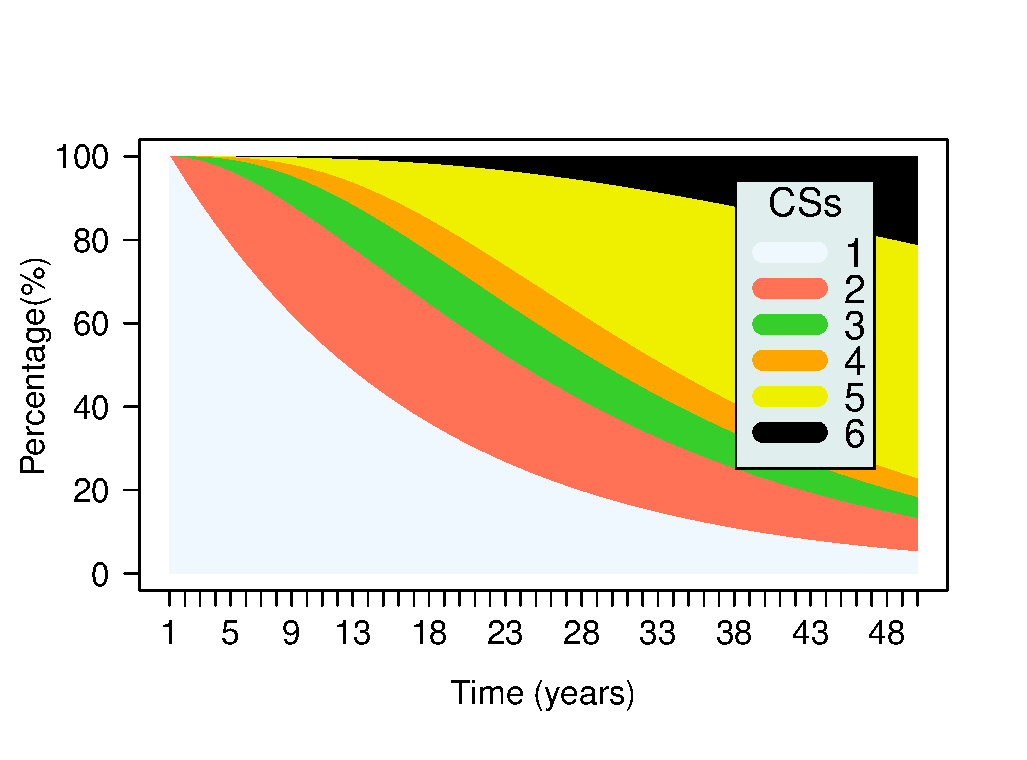
\includegraphics[width=0.8\linewidth]{csevolution}
    \caption{Evolution of states (manifest+latent)}
    \label{csevolution}
  \end{center}
\end{figure}

In Figure \ref{csevolution}, the black proportion infers the evolution of latent deterioration (state 6 or $l=1$). There is a gradual increase in the probability that the bridge will be in adequate LOS over time. This is because as the operational time of the bridge get longers, the bridge gets older and therefore, its reliability decreases. The multiplication of the state probability ($p_l^k$ in Equation (\ref{totalCIs}), $k=1$ as there is only one bridge) of the latent process and the unit impact ($Y$) mu of the corrective intervention for the bridge gives the expected total impact for respective year. This value will be a part of total corrective intervention impacts shown in Equation (\ref{totalCIs}).
%%%%
\subsection{Results}
Results of the example are shown in Figure \ref{results}. In the figure, the case corresponding to the thick red curve is considered as ``reference case'', in which, values of CI for the snow-barriers system and for the bridge are $X=2$ and $Y=10$, respectively.
\begin{figure}[H]
  \begin{center}
    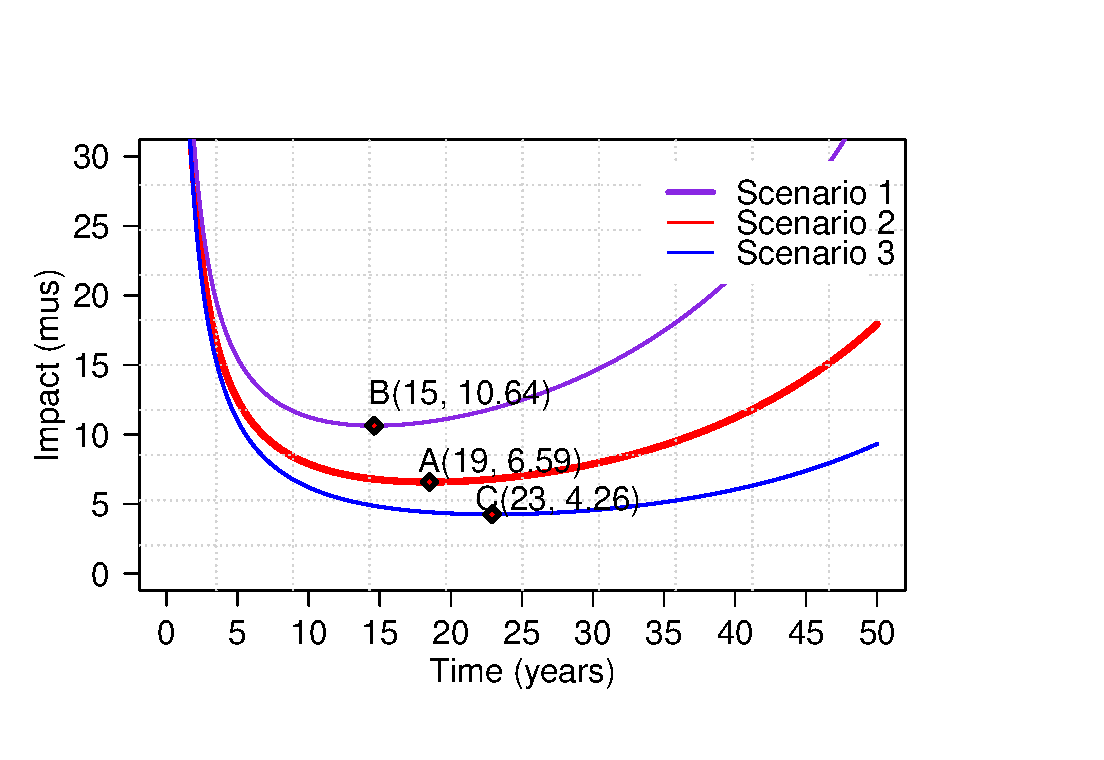
\includegraphics[width=0.8\linewidth]{results}
    \caption{Estimation results}
    \label{results}
  \end{center}
\end{figure}

For the reference case, the optimal time to execute a PI is at 19 year (point A) because if the PI is executed at that time, the annual impact will be minimal ($6.59$ $mus$). If either the PI is executed before or after that time, the annual impact will be higher. This is because if the PI is done earlier or more frequent, the impacts of executing PI will exponentially increase. On other hands, if the PI is executed less, the impacts incurred by executing CI will also exponentially increase. In a nutshell, there is an optimal time to execute the PI and this is important for infrastructure manager to know about it in order to be proactively prepared.

Also in the figure, there are purple curve and blue curve, which are drawns when implicitely selecting value of impact for executing CI for the snow-barries system to be twice more and twice less than that of the reference case. The purpose is to give a brief sensitivity analysis on the changes in the optimal time to execute an IS. It can be concluded that if the value of impact is more, the optimal time to execute the IS will be shorter (point B) than that of the reference case (point A) and vise versa (point C). The following section gives an indepth sensitivity analysis on the change in the ratio between PI and CI as well as on the change of parameters used in the model.
\section{Sensitivity analysis} \label{sa}
From the mathematical point of view, the optimal time to execute an IS depends on parameter values of reliability function used in both snow-barriers system and the bridge as well as the values of impacts incurred during the execution of an PI or an CI. However, values of coefficients and impacts cannot be precisely calculated. They are, however, subjected to uncertainties. It is therefore important to conduct a sensitivity analysis to understand the correlation in the changes of the optimal time to execute the PI and the changes of coefficients and impacts values. Following table gives an overview of criterias and ranges of their values used in the sensitivity analysis.
%

\begin{table}[h]
\begin{center}
 \caption{Ranges of values used for indicators and coefficients in the SA}
\begin{tabular}{l|c|cc}
\hline
\multirow{2}{*}{Criteria} & \multirow{2}{*}{Notation} & \multicolumn{2}{c}{Range of value} \\ \cline{3-4} 
 &  & \multicolumn{1}{l|}{Min} & \multicolumn{1}{l}{Max} \\ \hline
\multirow{2}{*}{Impact ratio} & $CI_{A}/PI$ & \multicolumn{1}{c|}{0.1} & 10 \\ \cline{2-4} 
 & $CI_{B}/PI$ & \multicolumn{1}{c|}{0.1} & 1'000 \\ \hline
\multirow{2}{*}{\begin{tabular}[c]{@{}l@{}}Reliability of\\ snow-barrier system\end{tabular}} & $\alpha$ & \multicolumn{1}{c|}{0.001} & 0.1 \\ \cline{2-4} 
 & $m$ & \multicolumn{1}{c|}{1} & 3 \\ \hline
\multirow{2}{*}{\begin{tabular}[c]{@{}l@{}}Reliability of\\ bridge\end{tabular}} & 100\% in state & \multicolumn{1}{c|}{1} & 5 \\ \cline{2-4} 
 & Avalanche intensity ($m^3$) & \multicolumn{1}{c|}{1} & 20 \\ \hline
Discount factor (\%) & $\rho$ & \multicolumn{1}{c|}{0} & 10 \\ \hline
\end{tabular}
\label{sensi}
\end{center}
\end{table}
The results of the SA for the impact ratio criteria are shown in graphs of Figure \ref{impactratio}.

\begin{figure}[ht!]
  \begin{center}
  \subfigure[$CI_A/PI$]
  	{
    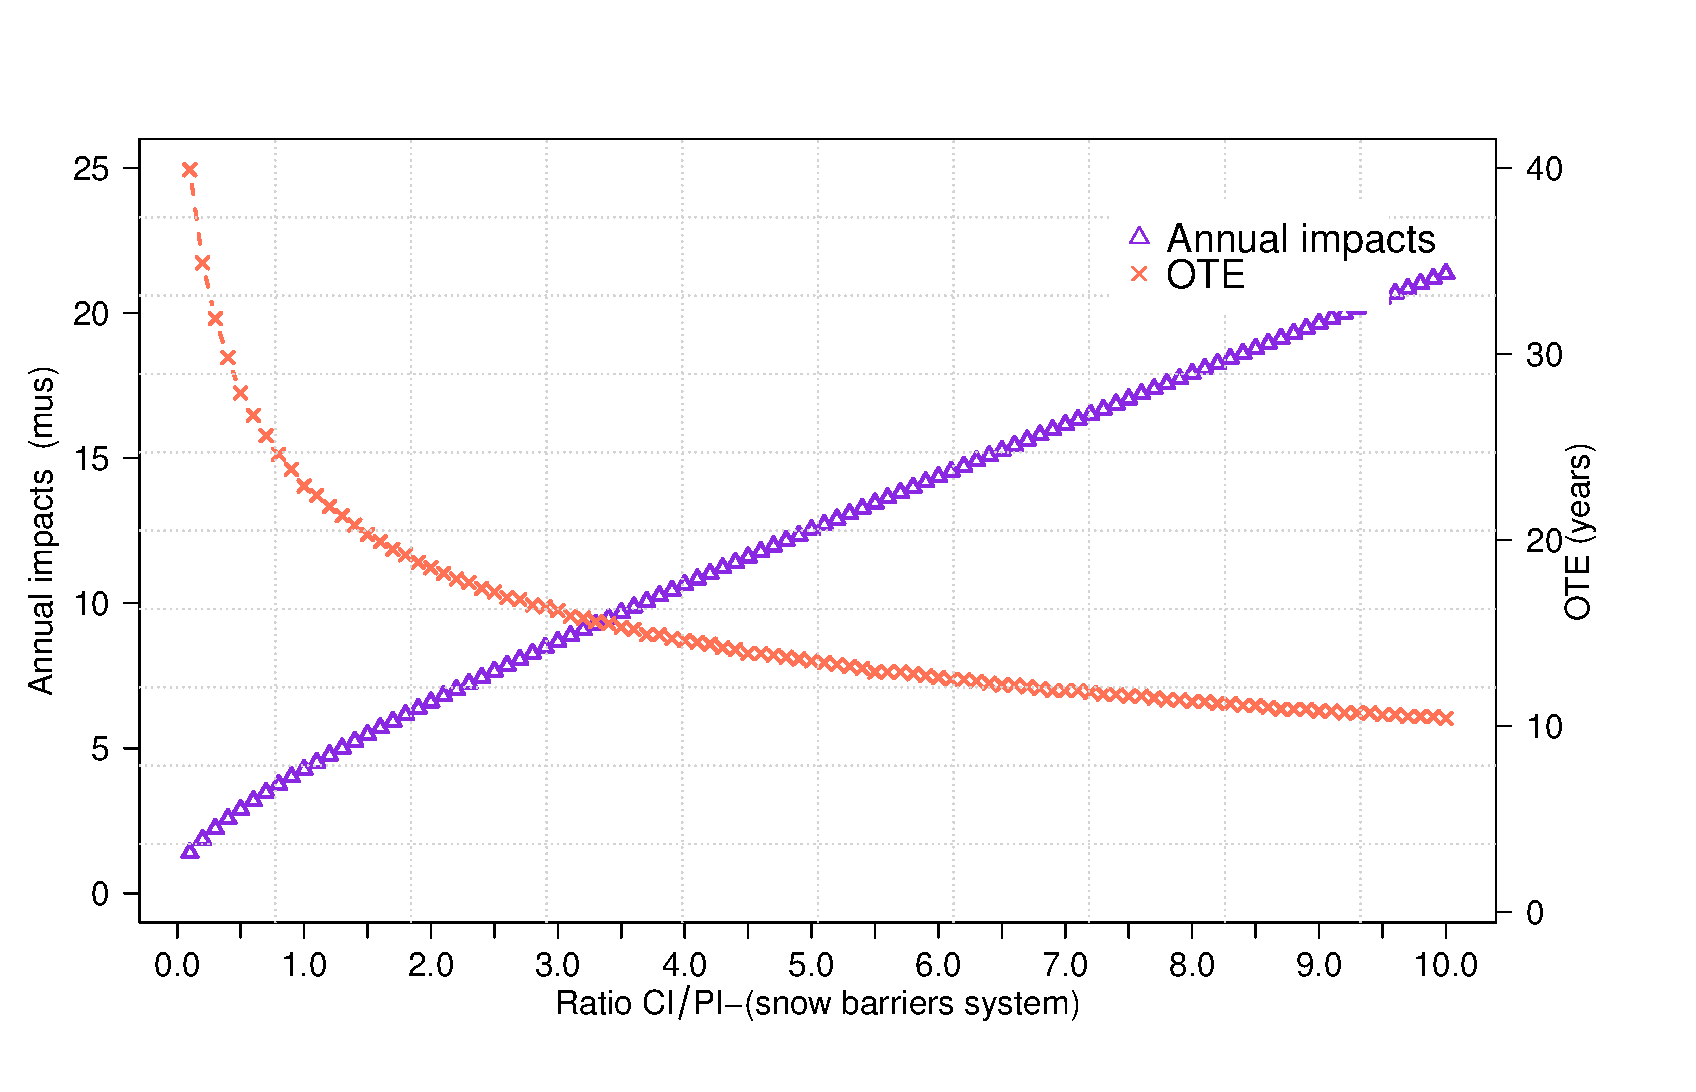
\includegraphics[width=0.4\linewidth]{snowbarrierssa}
    }
  \subfigure[$CI_B/PI$]
    {
      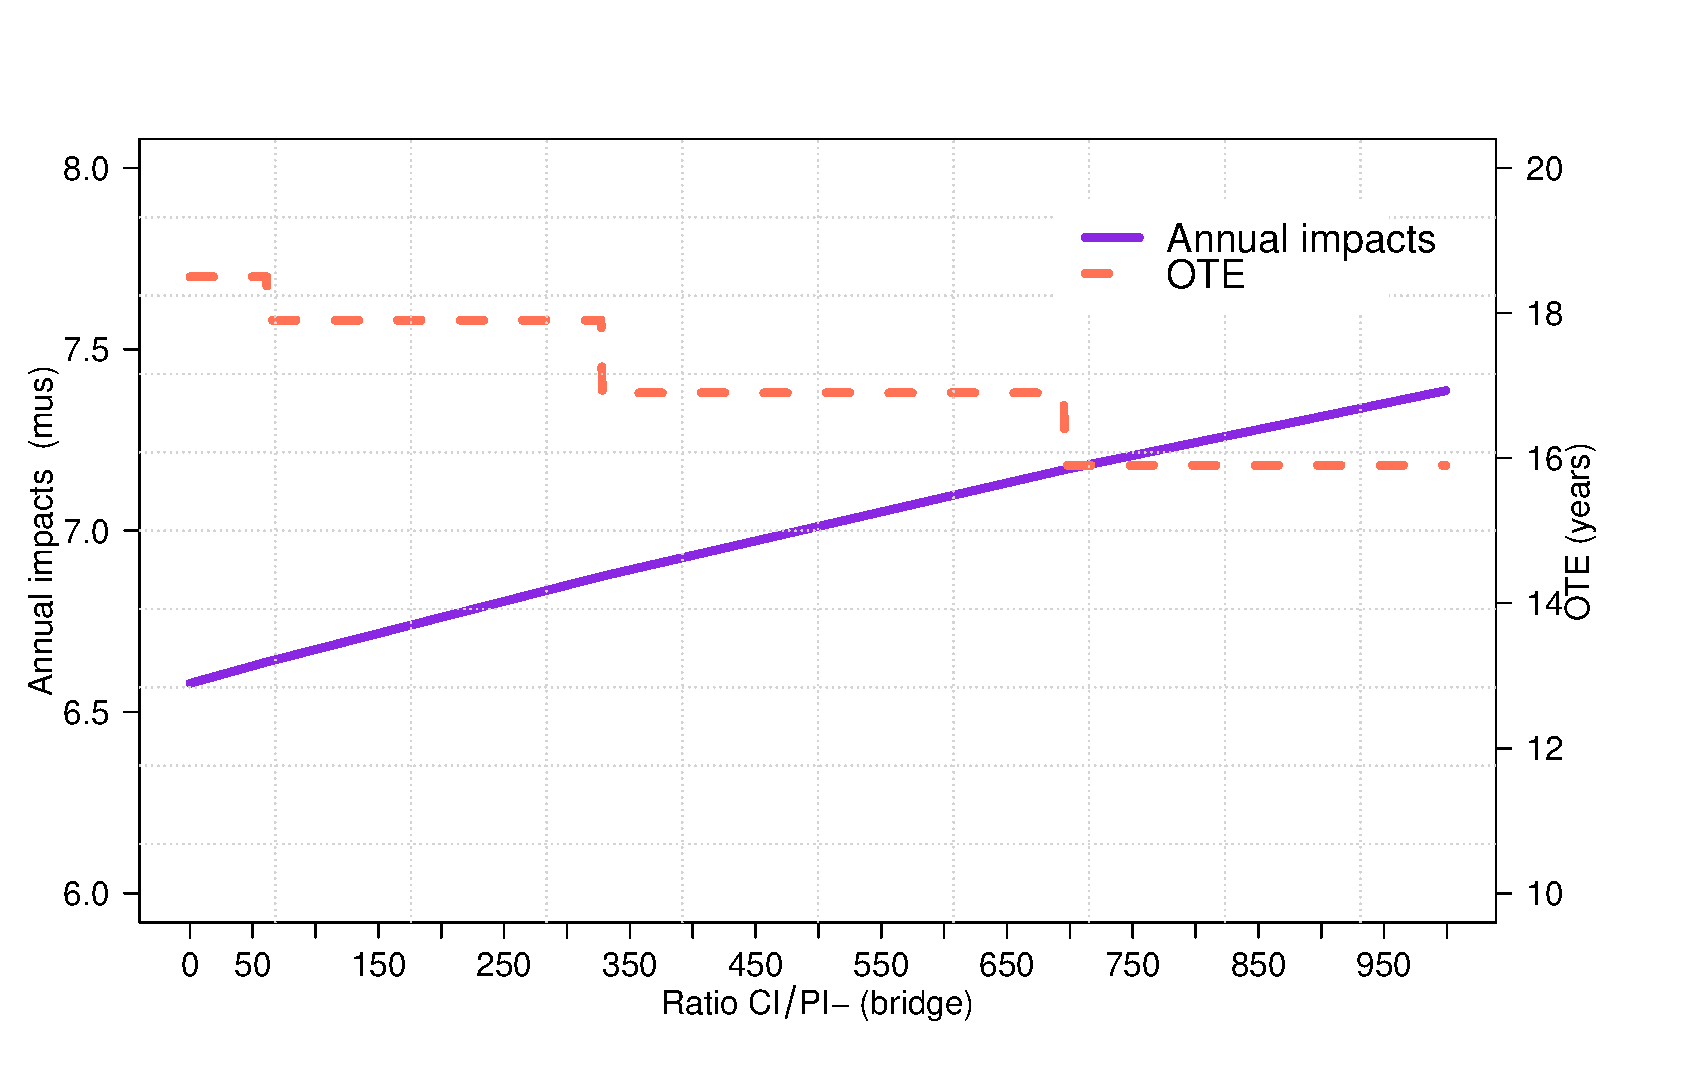
\includegraphics[width=0.4\linewidth]{steelbridgesa}
      }
    \caption{SA-impact ratio}
    \label{impactratio}
  \end{center}
\end{figure}


\begin{figure}[ht!]
  \begin{center}
  \subfigure[$\alpha$]
  	{
    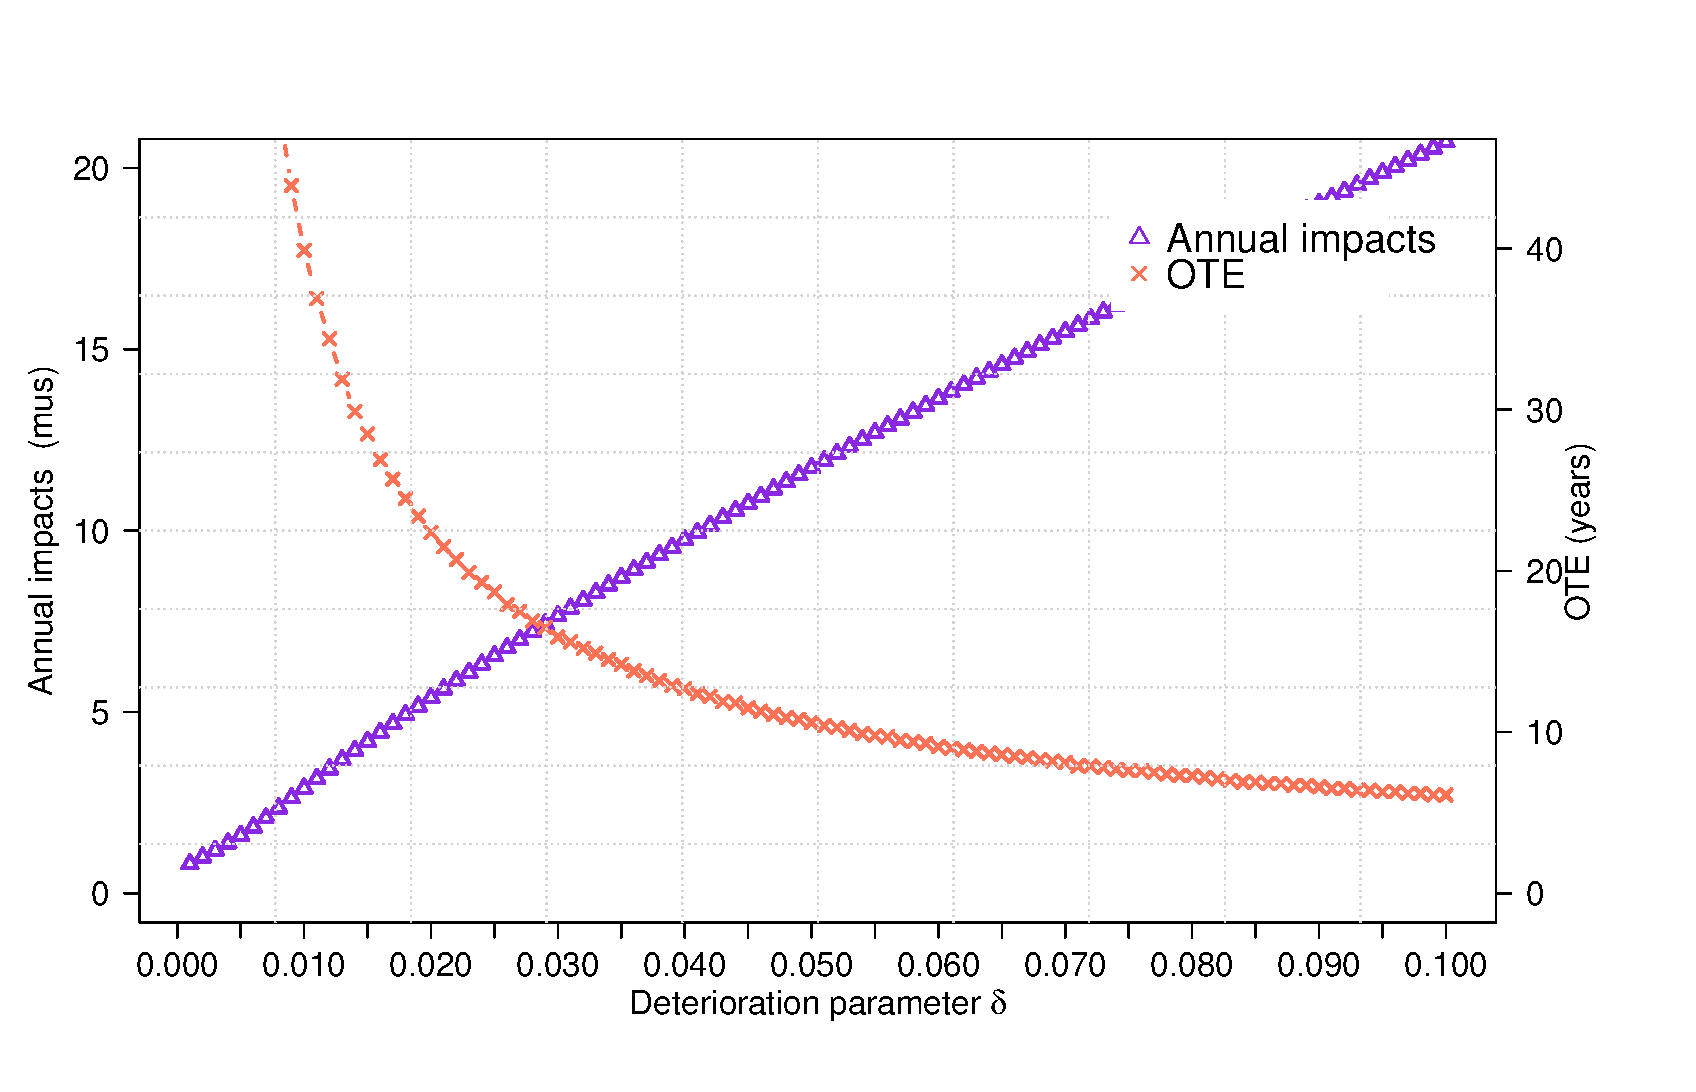
\includegraphics[width=0.4\linewidth]{alpha}
    }
  \subfigure[$m$]
    {
      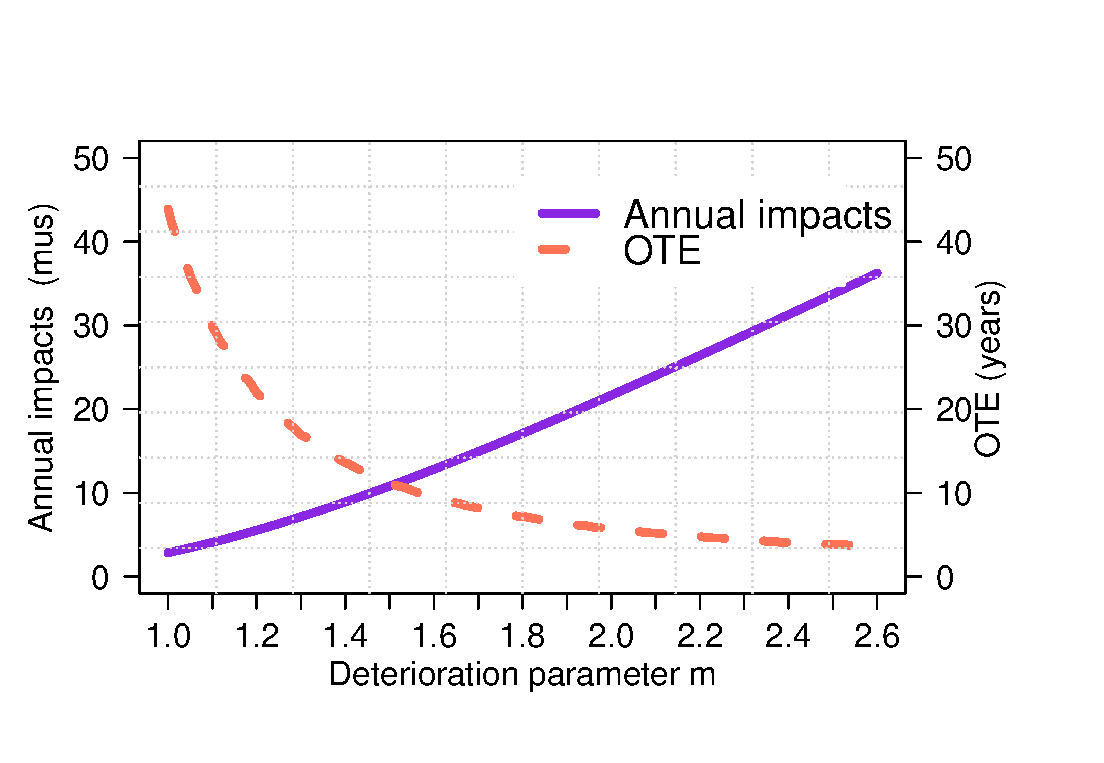
\includegraphics[width=0.4\linewidth]{m}
      }
    \caption{SA-reliability of the snow-barrier system}
    \label{reliabilitySPS}
  \end{center}
\end{figure}

\begin{figure}[ht!]
  \begin{center}
  \subfigure[Avalanche intensity]
  	{
    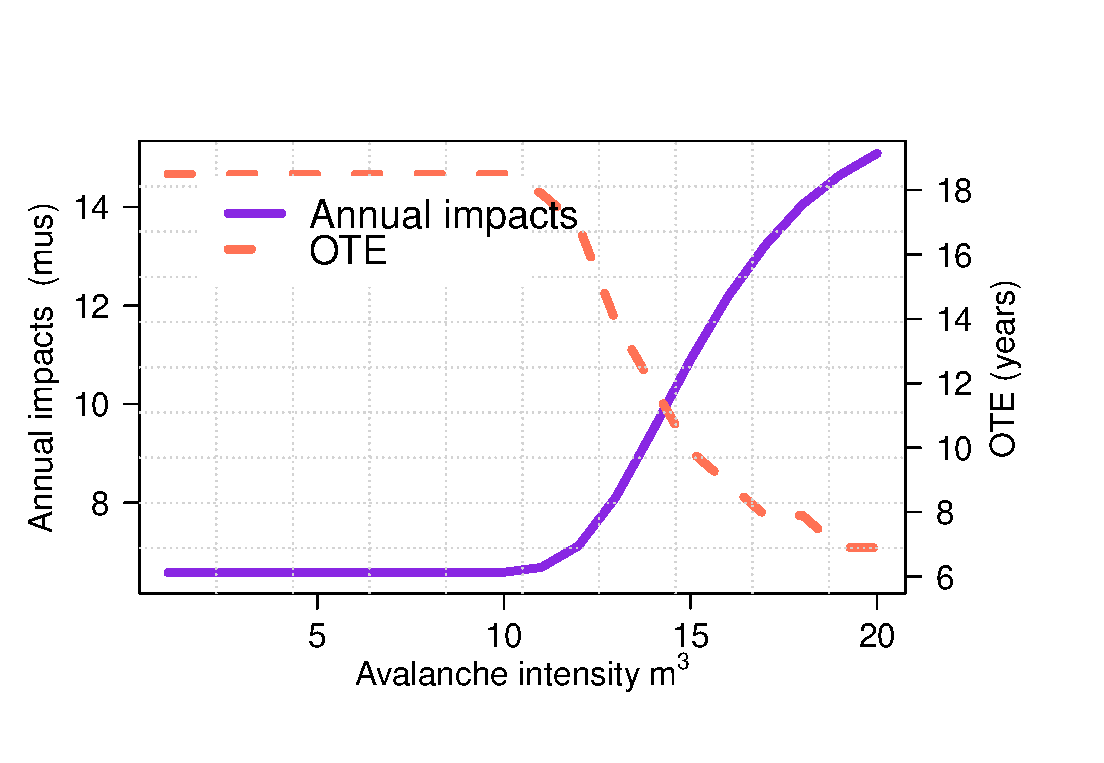
\includegraphics[width=0.4\linewidth]{avalancheintensity}
    }
  \subfigure[Age of bridge]
    {
      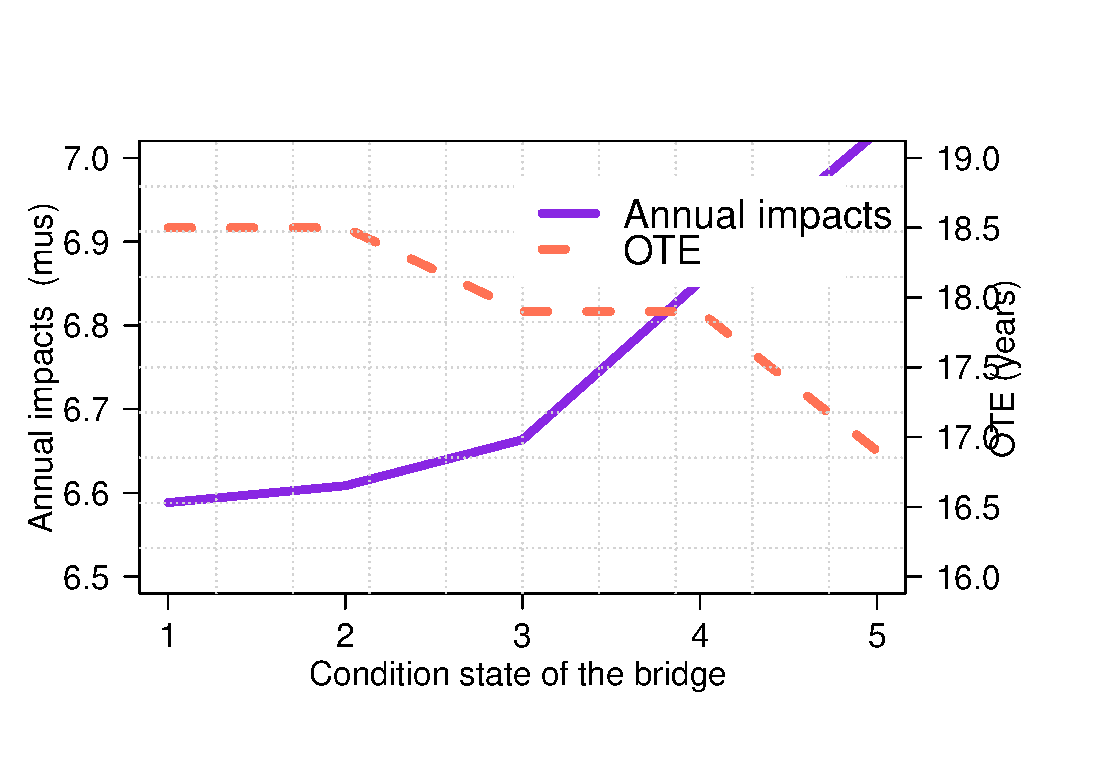
\includegraphics[width=0.4\linewidth]{bridgeCS}
      }
    \caption{SA-Avalanche intensity and state of the bridge}
    \label{reliabilitybridge}
  \end{center}
\end{figure}

\begin{figure}[ht!]
  \begin{center}
  %\subfigure[Discount factor]
  %	{
    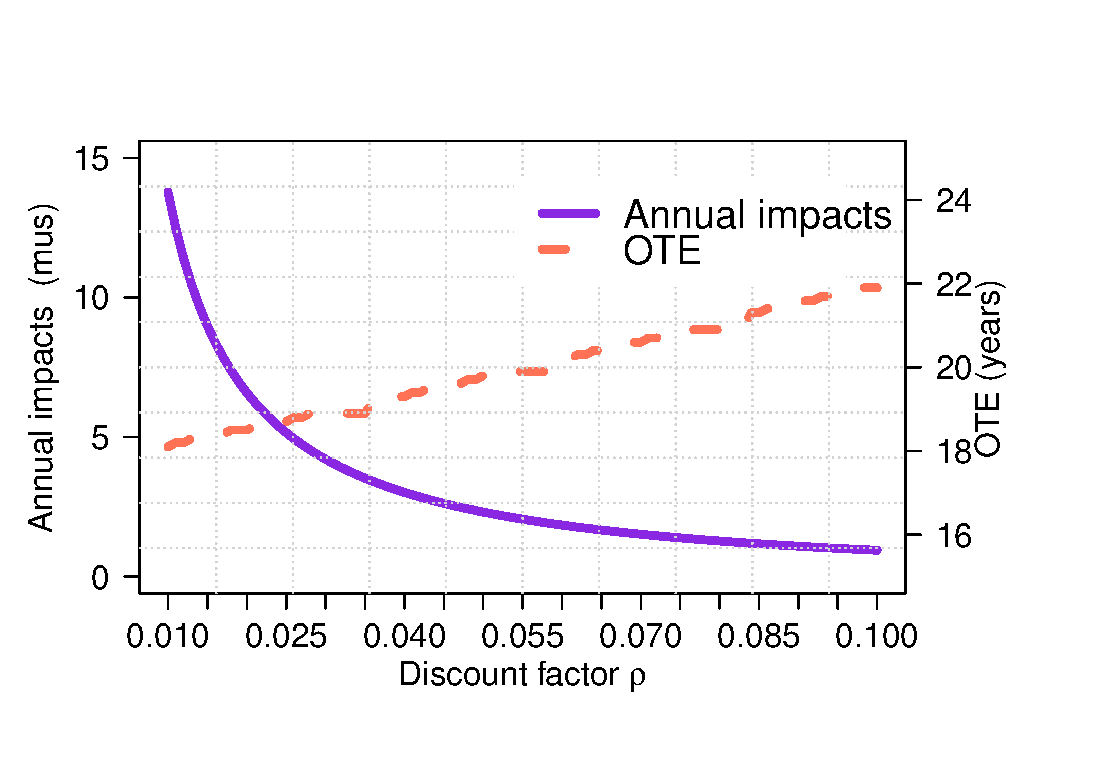
\includegraphics[width=0.4\linewidth]{discount}
   % }
    \caption{SA-Discount factor}
    \label{SAdiscount}
  \end{center}
\end{figure}

Following conclusions can be drawn by intepreting the changes in the optimal time to execute the PI with respect to different criteria

\begin{itemize}
 \item The lower the impact ratio is, the longer the optimal time to execute intervention (OTE) becomes (Figure \ref{impactratio}). The OTE is quite sensitive to the impact ratio ($CI_A/PI$), but not so sensitive to the impact ratio ($CI_B/PI$). This is because the impacts incurred by executing the CI for the snow-barriers system will dramatically change the reliability of the system itself. Whilst, the impact ratio $CI_B/PI$ has to be multipled with the transition probability of the latent state of the bridge, which is in fact significantly low in this example (Table \ref{totalmatrix} and Figure \ref{csevolution}),
 \item The OTE depends greatly on the values of parameters of the reliability function used for the snow-barrier system. As can be seen from Figure \ref{reliabilitySPS}, the OTE decreases nonliearly as values of $\alpha$ and $m$ increases. In the case of Weibul function, if value of $\alpha$ and $m$ increases, it means the rate of failure increases and therefore it is better to execute the PI earlier,
 \item The intensity of avalanche has a great influence on both the OTE and the annual impacts (Figure \ref{reliabilitybridge}-a) when it reaches to a certain threhold. For example, when the intensity of avalanche becomes more than 10 $m^3$, there is a sharp decreasing in the OTE and a sharp increasing in the value of impact. This is because, the bridge itself was designed to withstand a certain intensity of avalanche. However, if the intensity of avalanche reaches to a certain level, there is a higher chance that the bridge will be in adequate level of service. Under this circumstance, the value of CI on the bridge will plays an important part in determining the OTE. This finding is important for manager to carefully use the fragility curve for their objects by examining the most likely values of parameters of the fragility curves (e.g. values of $\alpha$ and $\gamma$ in Equation (\ref{fragility3})),
 \item The OTE depends also on actual state probability of the bridge. This conclusion can be confirmed with the curves shown in Figure \ref{reliabilitybridge}-b. The OTE tends is shorter when the state of the bridge gets worse (e.g. from being in state 1 to state 5). In this figure, the changes is not significant. However, it is not because the values of the state probability of the bridge but it is because the transition probability from manifest CS to latent Cs is really small. This is an interesting finding and convey an implication that managers, when determining the OTE for the snow-barrier system, they have to take into consideration of how the actual condition of other objects that being affected by the avalanche (e.g. the bridge),
 \item Changes in value of the discount factor is quite sensible to the change in the impact. However, it does not significantly change the value of OTE. In this example, the values of the discount factor was varied from 0 to 10\%, however, the difference of the OTE is only 4 years (Figure \ref{SAdiscount}). This is also an interesting point when managers consider to manage both the snow-barriers system and the bridge in a infinite time (e.g. long term management). Under an infinite case, the values of discount factor can be close to 0 (e.g. interest rate in developed nations is extremely small) or even can be ignored from the mathematical view points. This will make the numerical solution to the model more convenient.
\end{itemize}
\section{Conclusion} 
% % %
\label{conclusion}
In this paper, a reliability based methodology, which can be used to determine the optimal time to execute a preventive intervention for avalanche protection structures, is presented. The methodology is composed of an extended time dependent replacement model that can take into consideration of both finite and infinite time horizon and impacts incurred during the preventive intervention and corrective intervention of the avalanche protection structures. It also includes the discussion on the integration of existing fragility curves and Markov model used to model the manifest and latent deterioration of civil structures that could be in state of failure due to avalanche.

A numerical example was conducted for a snow-barriers system, which was installed in the starting zones of avalanche. The reliability of the system decreases over time and might fails to against avalanche. Consequently, avalanche might come into contact with a bridge and cause the bridge to be in inadequate level of service. Results of the example highlight important message to infrastructure managers of the avalanche protection system that the system should be replaced at an optimal time in order to minimize all negative impacts incurred by the stakeholders. The determination of the time is crucially dependent on the ratio of the impacts between the corrective intervention and preventive intervention as well as on the parameter values used to represent the reliability of the snow-barriers system. 

\bibliographystyle{plainnat} 
%\bibliographystyle{unsrt} 
\bibliography{reference}


%%%
\end{document}




